\documentclass{article}
\usepackage[utf8]{inputenc}
\usepackage[ngerman]{babel}
\usepackage{hyperref}
\usepackage[left=2cm, right=2cm, top=2cm, bottom=2cm]{geometry}
\usepackage{mathtools}
\usepackage{graphicx}
\usepackage{parskip}
\usepackage{float}
\usepackage{amsmath}
\usepackage{amsfonts}
\usepackage{amssymb}
\usepackage{blindtext}
\usepackage{array}
\usepackage{caption}
\usepackage{subcaption}
\usepackage{setspace}
\usepackage{siunitx}
\usepackage{xurl}
\onehalfspacing
\setlength{\parindent}{0em} 
\usepackage{csquotes}
\usepackage[style=ieee, backend=biber]{biblatex} % KORREKTE VERSION
\usepackage{booktabs}





\title{Pohlsches Rad}
\author{Bach Cao; Jakob Böhm \\ 
Team 2-3 \\
Technische Universität München}
\date{01.04.2025}


\begin{document}

\maketitle
\pagenumbering{gobble}


\tableofcontents
\pagenumbering{gobble}
\newpage

\pagenumbering{arabic} 
\setcounter{page}{1}
%----------------------------------------------------------------------------------------------------

\section{Einleitung}
In diesem Versuch wird das Schwingungsverhalten eines speziellen Drehpendels, des Pohlschen Rades, untersucht. Zunächst werden die Eigenfrequenz und die Dämpfungskonstante anhand einer gedämpften freien Schwingung bestimmt. Anschließend wird die Resonanzfrequenz ermittelt, indem das System durch äußere Erregung mit verschiedenen Frequenzen zu erzwungenen Schwingungen angeregt wird.




%----------------------------------------------------------------------------------------------------
\vspace{1cm}  
\section{Theoretische Grundlagen}

Im Folgenden werden nur lineare Systeme betrachtet, deren Bewegungsgleichung eine lineare Differentialgleichung ist.



\subsection{Freie gedämpfte Schwingung}
Ein nicht angetriebenes Pendel, welches um seine Ruhelage schwingt und dabei Energie verliert, führt eine gedämpfte Eigenschwingung aus, welche durch die Bewegungsgleichung

\begin{equation}
    \Theta \ddot{\varphi} + \gamma \dot{\varphi} + k \varphi = 0
\end{equation}

beschrieben werden kann. Dabei ist $\Theta$ das Trägheitsmoment des Pendels, $\varphi$ die Auslenkung, $\gamma$ das Dämpfungsmoment und $k$ das rücktreibende Moment der Feder. Für das verwendete Pendel ist die Dämpfungskonstante $\lambda = \frac{\gamma}{2\Theta}$ sinnvoll. Es wird nur der Fall schwacher Dämpfung betrachtet $(\lambda^2 < k/\Theta)$. Die Lösung der Bewegungsgleichung hierfür lautet

\begin{equation}
    \varphi(t) = \varphi_0 \cdot e^{-\lambda t} \cos(\omega_d t + \delta) ,
\end{equation}

wobei $\varphi_0$ die Anfangsauslenkung, $\delta$ die Phasenverschiebung und $\omega_d = \sqrt{\frac{k}{\Theta} - \lambda^2}$ die Eigenkreisfrequenz der gedämpften Schwingung ist. Der Exponentialterm beschreibt die Dämpfung, welche durch die Abklingzeit

\begin{equation}
    \tau = \frac{1}{\lambda}
\end{equation}

und die Eigenfrequenz

\begin{equation}
    f = \frac{\omega_d}{2\pi}
\end{equation}

charakterisiert. Es ergibt sich folgende Funktion:

\begin{figure}[H]
    \centering
    \includegraphics[width=0.5\textwidth]{gedämpfte_Schwingung.jpg}
    \caption{Realteil der Lösung der Bewegungsgleichung für den Fall von schwacher Dämpfung [1].}
    \label{fig:gedämpfte_Schwingung}
\end{figure}



\subsection{Resonanzkurve}
Ein externes Drehmoment $M_0 \sin(\omega t)$ führt zu erzwungenen Schwingungen, welche durch die modifizierte Bewegungsgleichung 

\begin{equation}
    \Theta \ddot{\varphi} + \gamma \dot{\varphi} + k \varphi = M_0 \sin(\omega t).
\end{equation}

mit der partikulären Lösung

\begin{equation}
    \varphi_p (t) = A(\omega) \sin(\omega t - \delta)
\end{equation}

dargestellt werden kann, wobei die Amplitude

\begin{equation}
    A(\omega) = \frac{M_0}{\Theta \sqrt{(\omega_0^2 - \omega^2)^2 + 4\lambda^2 \omega^2}}
\end{equation}

gegeben ist.

Hierbei ist $\omega_0 = \sqrt{k/\Theta}$ die Eigenfrequenz des ungedämpften Pendels. Die maximale Amplitude tritt bei der Resonanzfrequenz

\begin{equation}
    \omega_R = \sqrt{\frac{k}{\Theta} - 2\lambda^2}
    \label{Gleichung8}
\end{equation}

auf. Die Halbwertsbreite $\Delta\omega$ der Resonanzkurve ergibt sich für schwache Dämpfung zu:

\begin{equation}
    \Delta\omega = \lambda.
    \label{9}
\end{equation}


\begin{figure}[H]
    \centering
    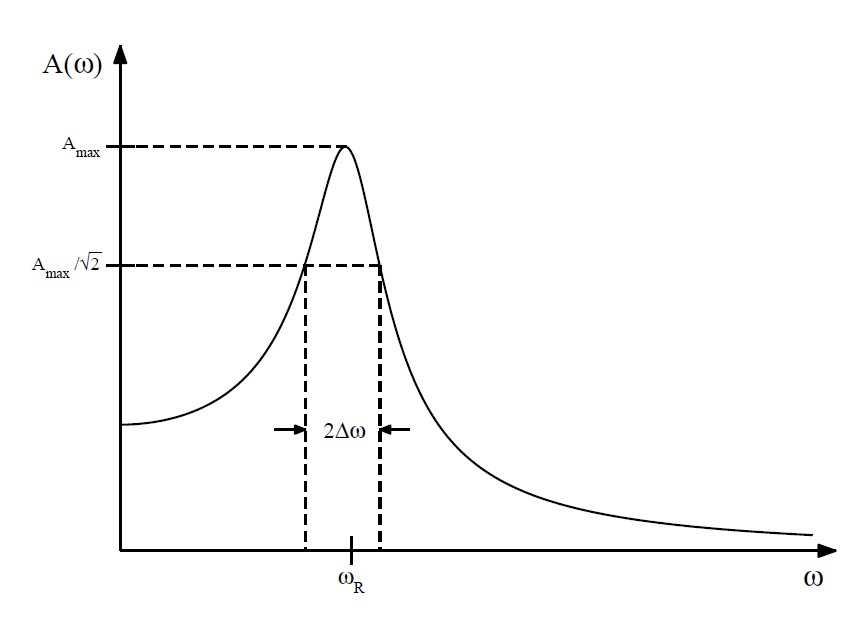
\includegraphics[width=0.6\textwidth]{Resonanzkurve.jpg}
    \caption{Resonanzkurve mit eingezeichneter Halbwertsbreite[1].}
    \label{fig:Resonanzkurve}
\end{figure}




%----------------------------------------------------------------------------------------------------
\vspace{1cm}  
\section{Experimentelles Vorgehen}
Das Pohlsche Rad ist ein spezielles Drehpendel mit einer drehbaren Kupferscheibe, deren Ruhelage durch eine Spiralfeder bestimmt wird. Die Auslenkung kann auf einer Skala abgelesen werden.



\section{Gedämpfte Oszillation mit gleichbleibendem Dämpfungsstrom}

\subsection{Freie gedämpfte Schwingung}
\subsubsection{Bestimmung der Eigenfrequenz}
\label{4.1.1}

Im ersten Teil des Versuchs wurde die Schwingungsperiode bestimmt, indem insgesamt fünfmal die Zeit für zehn Schwingungen mit einer Stoppuhr gemessen wurde. Die Dämpfung erfolgt über eine Wirbelstrombremse, deren Stärke durch einen variablen Strom (bei uns $I = (0.432 \pm 0,001)$A) geregelt wird.

Zudem wurden die Maximalamplituden jeder Schwingung aufgezeichnet. Hierbei entsprechen $180$° insgesamt $25$ Skaleneinheiten am Pohlschen Rad bzw. $98,15$ Skaleneinheiten im Computerprogramm. Die Periodendauer berechnet sich aus

\begin{equation}
    T = \frac{T_{10}}{10}
\end{equation}

mit $T_{10} = (20,28 \pm 0,50)$s zu

\begin{equation}
    T = (2,028 \pm 0,05) \text{ s}.
\end{equation}

Daraus folgt die Eigenfrequenz

\begin{equation}
    \omega_m = \frac{2\pi}{T} = (3,098 \pm 0,076) \text{s}^{-1}
\end{equation}

Zum Vergleich wurde die Messung zusätzlich mit Hilfe von Cassy Lab ausgewertet. Dabei trägt der Computer in Abbildung \ref{fig:voltage_time} die Auslenkung gegen die Zeit auf. Eine Auftragung für ausschließlich der Amplituden von Computerdaten wäre hier nicht geeignet, weil sie nach jeder Schwingung manuell bestimmen werden müssten. Die halblogarithmische Auftragung wird ausschließlich für manuell notierten Daten verwendet, weil Logarithmus nicht definiert wird für negativen Bereich, der wegen des harmonischen Verhaltens bei Computerdaten auftritt. Hierbei ergibt sich die Eigenfrequenz des Pohlschen Rades zu

\begin{equation}
\omega_c = (3.1155 \pm 0.0012) \text{ s}^{-1}
\end{equation}

ergibt. Das manuell gemessene Ergebnis für $\omega_m$ stimmt mit dem gefitteten $\omega_c$ innerhalb der Unsicherheiten überein. Die Unsicherheit des Parameters von dem Fit wurde mithilfe der Kovarianzmatrix berechnet.

\begin{figure}[H]
    \centering
    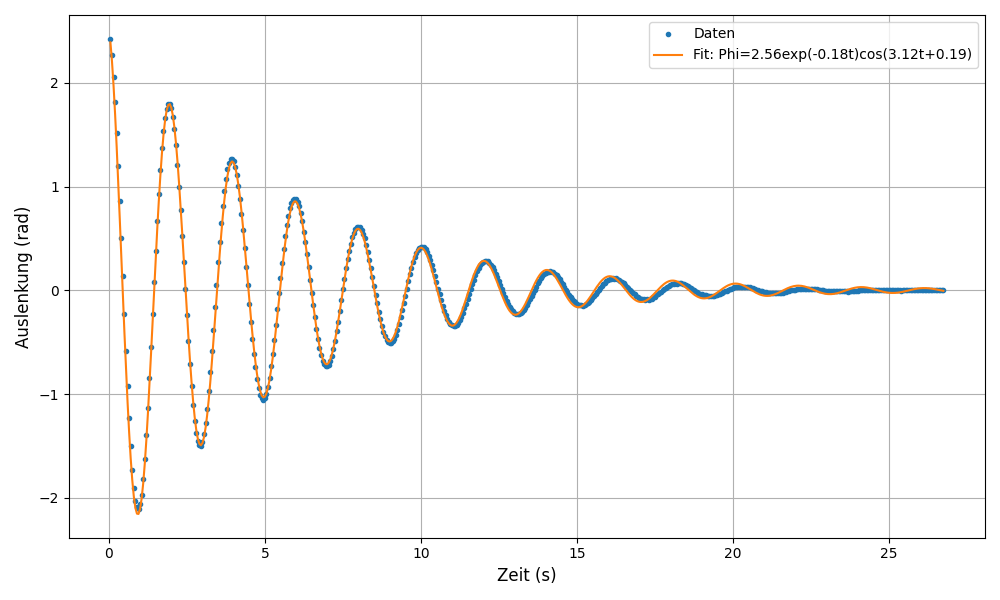
\includegraphics[width=0.7\textwidth]{Figure_11.png}
    \caption{Computer-Messung: Auslenkung über die Zeit aufgetragen}
    \label{fig:voltage_time}
\end{figure}

\subsubsection{Bestimmung der Dämpfungskonstante}
Das Pendel wird aus der Ruhelage bis zum Maximum ausgelenkt und schwingt anschließend bis zum Stillstand. Abbildung \ref{fig:max_amplitude} trägt halblogarithmisch die manuell notierten Amplituden gegen die Zeit auf.  Nach jeder Schwingung wird die maximale Amplitude abgeschätzt und dokumentiert. Daraus ergibt sich die Dämpfungskonstante als die Steigung der Fitgeraden $\lambda = 0,1873 \pm 0,0021$ $\text{s}^{-1}$. Die entsprechende Abklingzeit ist daher $\tau = \frac{1}{\lambda} = 5,343\pm0,062 \si{\second}$. Um die Schätzwerte vergleichen zu können, verwenden wir wiederum den Fit aus Abbildung \ref{fig:voltage_time}, wobei die Dämpfungskonstante als $\lambda = 0,1830 \pm 0,0012$ $\text{s}^{-1}$ bestimmt wurde. Die Abklingzeit entspricht daher $\tau = \frac{1}{\lambda} = 5,464\pm0,036 \si{\second}$. Zwar stimmen die Werte innerhalb der Unsicherheiten nicht überein, ist die Abweichung erst nach zwei Nachkommastellen festzustellen. Dies lässt sich durch Ablese-und-Zeitmessfehler begründen.


\begin{figure}[H]
    \centering
    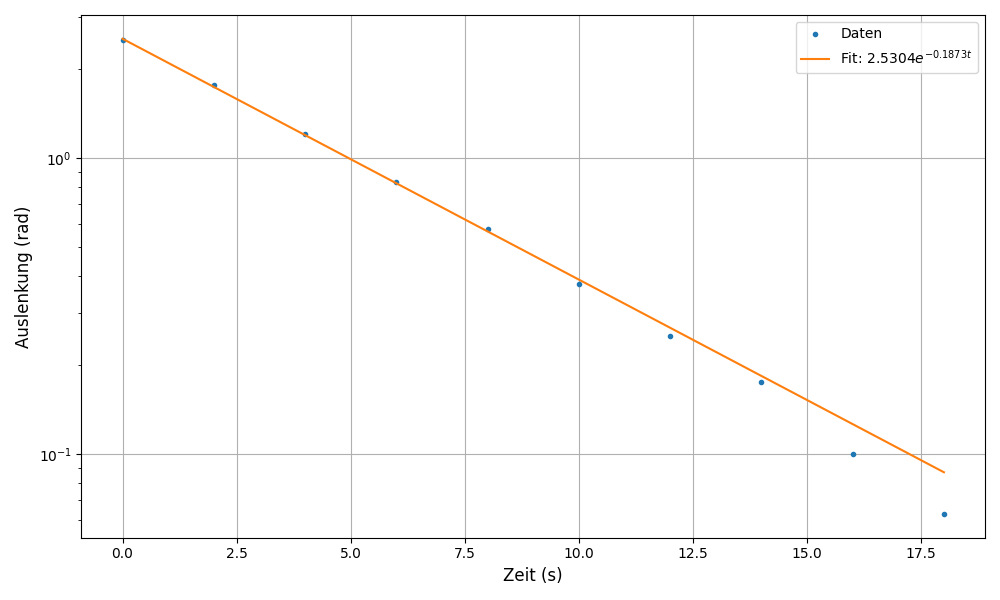
\includegraphics[width=0.7\textwidth]{Figure_12.png}
    \caption{Maximale Amplitude halblogarithmisch aufgetragen gegen die Zeit}
    \label{fig:max_amplitude}
\end{figure}

\subsubsection{Erzwungene gedämpfte Schwingung}
Im zweiten Teil des Experiments treibt ein Motor das Pendel zu Schwingungen mit einer bestimmten Frequenz an. Die Anregungsfrequenz wird langsam erhöht, wobei die maximale Amplitude aufgezeichnet wird. In der Nähe der Resonanz werden kleinere Frequenzsprünge verwendet. Die Auftragung der maximalen Amplitude gegen die Frequenz wird in \ref{fig:resonanz} durchgeführt.

\begin{figure}[H]
    \centering
    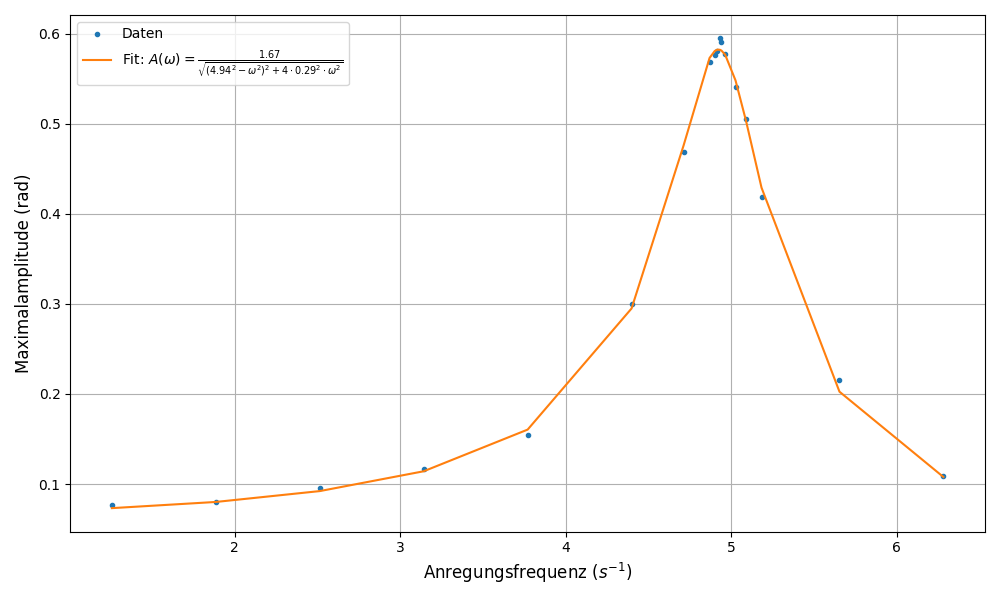
\includegraphics[width=0.7\textwidth]{Figure_13.png}
    \caption{Maximale Amplitude aufgetragen gegen die Anregungsfrequenz}
    \label{fig:resonanz}
\end{figure}

Dabei ist auffällig, dass bei gleicher Stromstärke eine starke Abweichung der Dämpfungskonstante mit dem berechneten Wert auftritt: $\lambda = 0,29 \pm 0,01$ $\text{s}^{-1}$. Die aufgenommenen Daten sind daher unpassend für die Auswertung, weil für kleiner Stromstärke die Resonanzfrequenz mit der Eigenfrequenz übereinstimmen sollte. Hierbei wurde Datenquelle von einem virtuellen Versuch benutzt [2]. Erneut werden in Abbildung \ref{fig:resonanz2} die neuen Daten aufgetragen.

\begin{figure}[H]
    \centering
    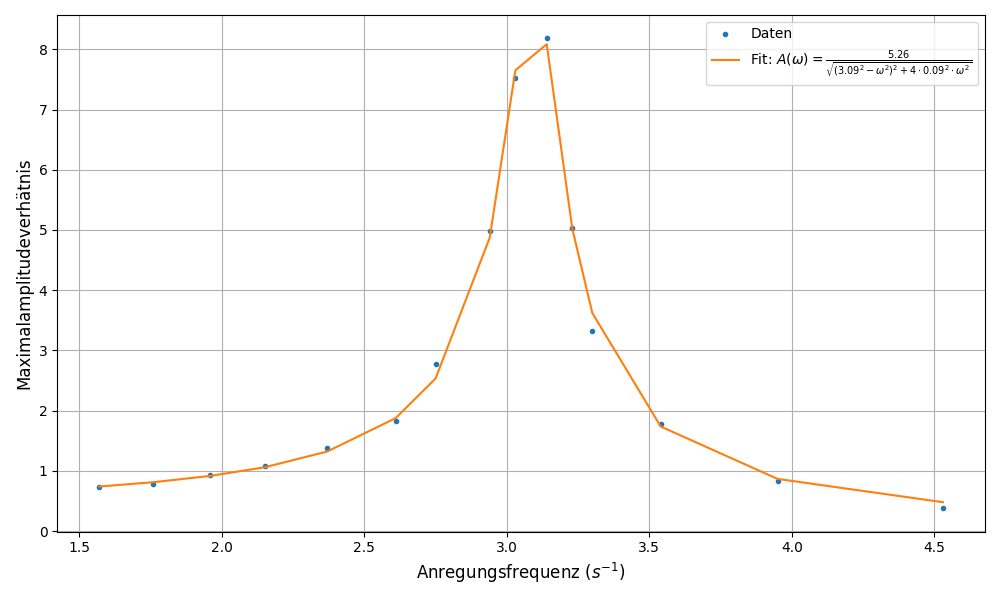
\includegraphics[width=0.7\textwidth]{Figure_14.png}
    \caption{Maximale Amplitude aufgetragen gegen die Anregungsfrequenz}
    \label{fig:resonanz2}
\end{figure}

Daraus ergibt sich die Resonanzfrequenz $\omega = 3,0942\pm 0,0020$ $\text{s}^{-1}$, was innerhalb Unsicherheiten mit (dem gebildeten Mittelwert) der berechneten Eigenfrequenz des Systems aus Abschnitt  \ref{4.1.1} übereinstimmt. Das liegt daran, dass bei dem virtuellen Versuch auch eine kleine Stromstärke bei $\SI{0,35}{\ampere}$ benutzt wurde. Daher ist die Abweichung der Resonanzfrequenz von der Eigenfrequenz auch vernachlässigbar. Daraus erhält man

\begin{equation}
\Delta \omega = (0.1013 \pm 0.009) \text{ s}^{-1}
\end{equation}

Aus dem Fit liest man die Dämpfungskonstante ab:  $\lambda = 0,0930 \pm 0,0031$ $\text{s}^{-1}$. Es stimmt innerhalb der Unsicherheiten mit der Halbwertsbreite überein. Damit ist Gleichung \ref{9} erfüllt.


\section{Gedämpfte Oszillation mit unterschiedlichen Dämpfungsströmen}

\subsection{Bestimmung der Dämpfungskonstante}
In diesem Unterversuch wird der Dämpfungsstrom zwischen 0,2 A und 1,5 A variiert. Ziel dieses Versuchs ist es, einen Zusammenhang zwischen der Dämpfungskonstante und dem Dämpfungsstrom sowie der Eigenfrequenz zu finden. Um dieses Ziel zu erreichen, müssen die Messungen der Schwingungen mit verschiedenen Dämpfungsströmen angepasst werden. Die Ergebnisse für die Eigenfrequenz und die Dämpfungskonstante in Abhängigkeit vom Dämpfungsstrom sind in Tabelle \ref{tab:fit} dargestellt.

\begin{table}[H]
    \centering
    \begin{tabular}{c|c|c}
        \toprule
        $I$ [A] & $\lambda$ [$\text{s}^{-1}$] & $\omega$ [$\text{s}^{-1}$] \\
        \midrule
        $0.200\pm0.005$ & 0.05 & 3.13 \\
        $0.300\pm0.005$ & 0.10 & 3.11 \\
        $0.400\pm0.005$ & 0.16 & 3.11 \\
        $0.499\pm0.005$ & 0.25 & 3.09 \\
        $0.600\pm0.005$ & 0.35 & 3.07 \\
        $0.700\pm0.005$ & 0.46 & 3.08 \\
        $0.800\pm0.005$ & 0.59 & 3.03 \\
        $0.894\pm0.005$ & 0.73 & 3.04 \\
        $1.002\pm0.005$ & 0.92 & 2.99 \\
        $1.099\pm0.005$ & 1.12 & 2.92 \\
        $1.199\pm0.005$ & 1.32 & 2.82 \\
        $1.299\pm0.005$ & 1.56 & 2.68 \\
        $1.396\pm0.005$ & 1.82 & 2.49 \\
        $1.502\pm0.005$ & 2.10 & 2.30 \\
        \bottomrule
    \end{tabular}
    \caption{Aus dem Fit ermittelte Dämpfungskonstante und Eigenfrequenz von jeweiligem Dämpfungsstrom. Im Anhang werden die Fits beigefügt.}
    \label{tab:fit}
\end{table}
In Abbildung \ref{fig:Dämpfungskonstante} wird die Dämpfungskonstanten gegen die Dämpfungsströme aufgetragen. Die quadratische Abhängigkeit lässt sich deutlich erkennen.

\begin{figure}[H]
    \centering
    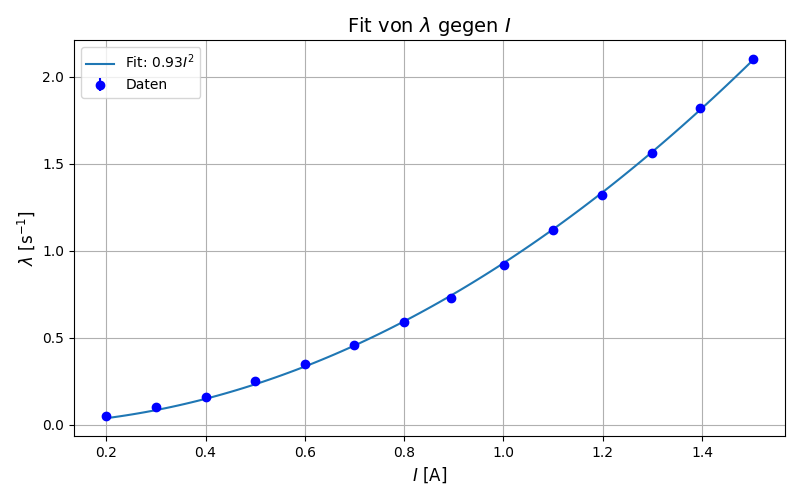
\includegraphics[width=0.7\textwidth]{Figure_8.png}
    \caption{Dämpfungskonstante in Abhängigkeit des Dämpfungsstroms.}
    \label{fig:Dämpfungskonstante}
\end{figure}



\subsection{Eigenfrequenz in Abhängigkeit der Dämpfungskonstante}

In diesem Unterkapitel werden die Ergebnisse für die Eigenfrequenzen in Abhängigkeit von der Dämpfungskonstante, die im vorherigen Unterkapitel ermittelt wurden, in Grafik \ref{fig:Eigenfrequenz} grafisch dargestellt und diskutiert.

\begin{figure}[H]
    \centering
    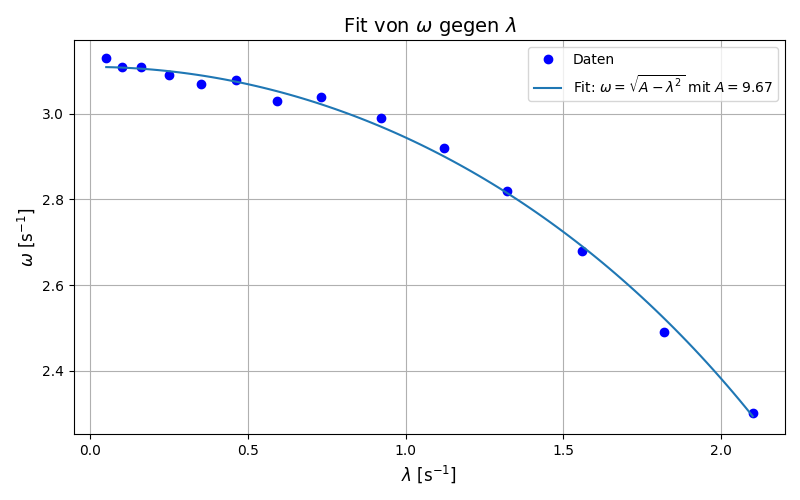
\includegraphics[width=0.7\textwidth]{Figure_10.png}
    \caption{Eigenfrequenz in Abhängigkeit der Dämpfungskonstante}
    \label{fig:Eigenfrequenz}
\end{figure}

Wie zu erwarten, nimmt die Eigenfrequenz mit zunehmender Dämpfungskonstante ab. Das Verhalten stimmt gut mit dem theoretisch zu erwartenden gut überein. Der für den Fit verwendete Parameter repräsentiert die Größe $\frac{k}{\Theta}$. Die kleinen Abweichungen der Datenpunkten lassen sich wahrscheinlich durch Umrechnungsfehler oder Detektorungenauigkeit von Cassylab begründen.

\section{Anhang}

Im Folgenden werden die Datenanpassungen für die Messungen aller Dämpfungsströme beigefügt.

\begin{figure}[H]
    \centering
    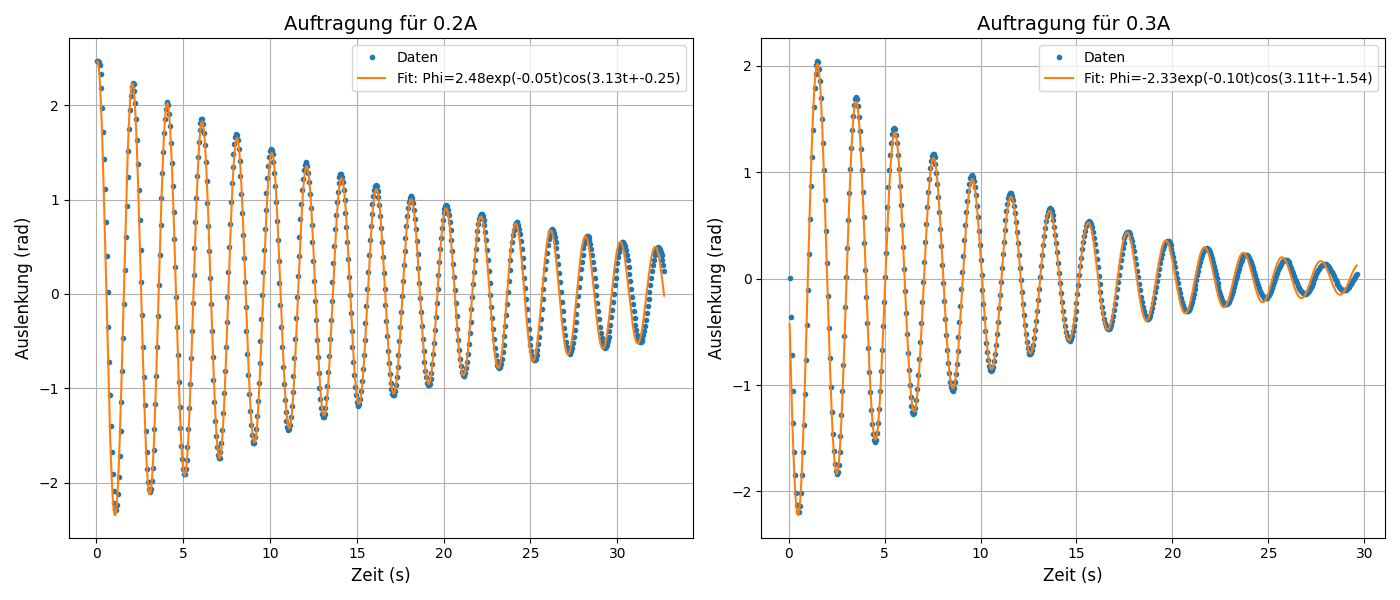
\includegraphics[width=0.85\textwidth]{Figure_1.png}
    \caption{Datenanpassung für Dämpfungsströme (1).}
    \label{fig:1}
\end{figure}
\begin{figure}[H]
    \centering
    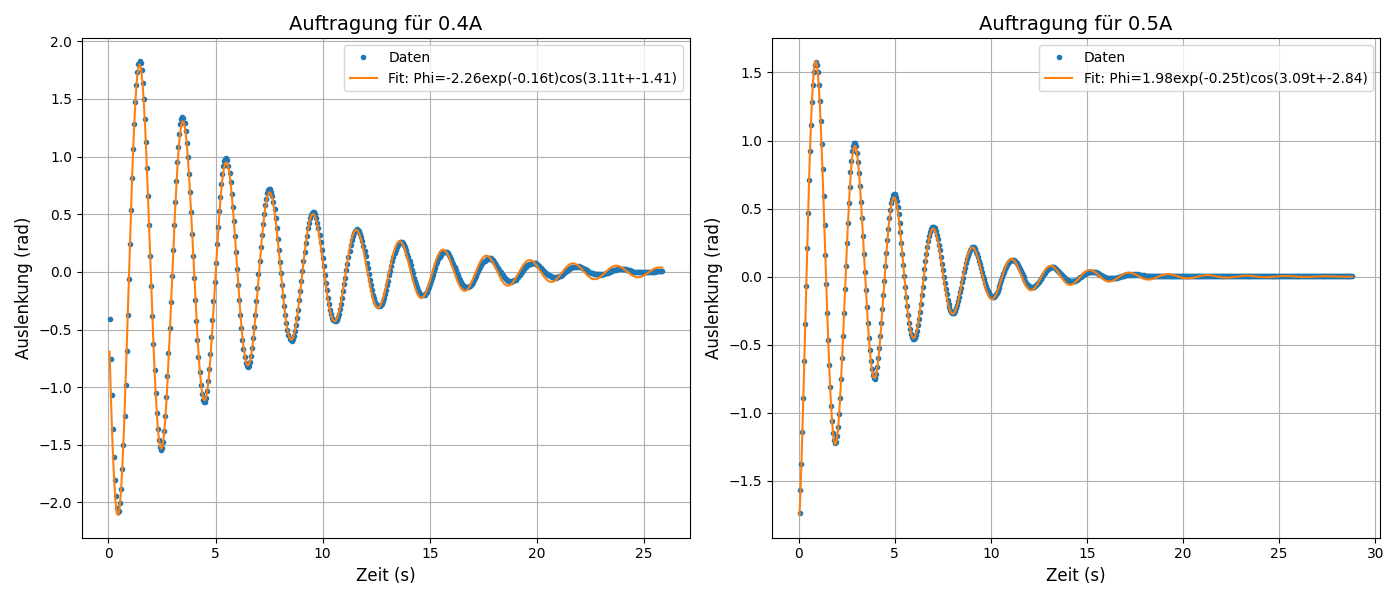
\includegraphics[width=0.85\textwidth]{Figure_2.png}
    \caption{Datenanpassung für Dämpfungsströme (2).}
    \label{fig:2}
\end{figure}
\begin{figure}[H]
    \centering
    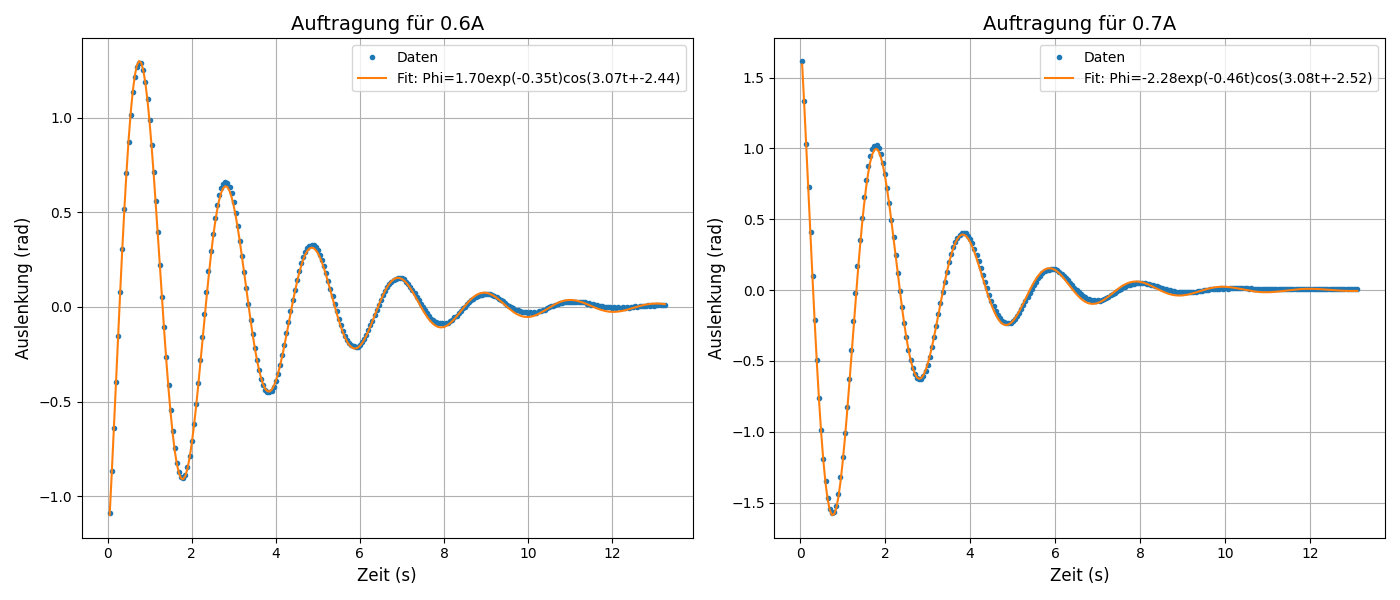
\includegraphics[width=0.85\textwidth]{Figure_3.png}
    \caption{Datenanpassung für Dämpfungsströme (3).}
    \label{fig:3}
\end{figure}
\begin{figure}[H]
    \centering
    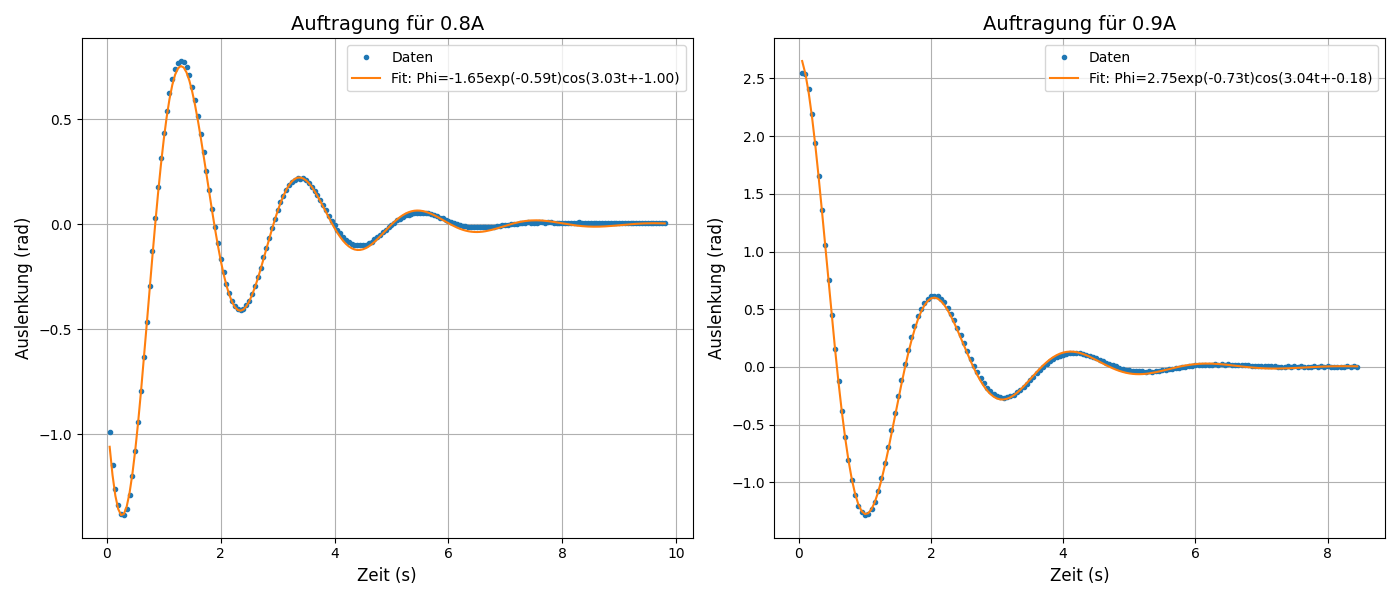
\includegraphics[width=0.85\textwidth]{Figure_4.png}
    \caption{Datenanpassung für Dämpfungsströme (3).}
    \label{fig:4}
\end{figure}
\begin{figure}[H]
    \centering
    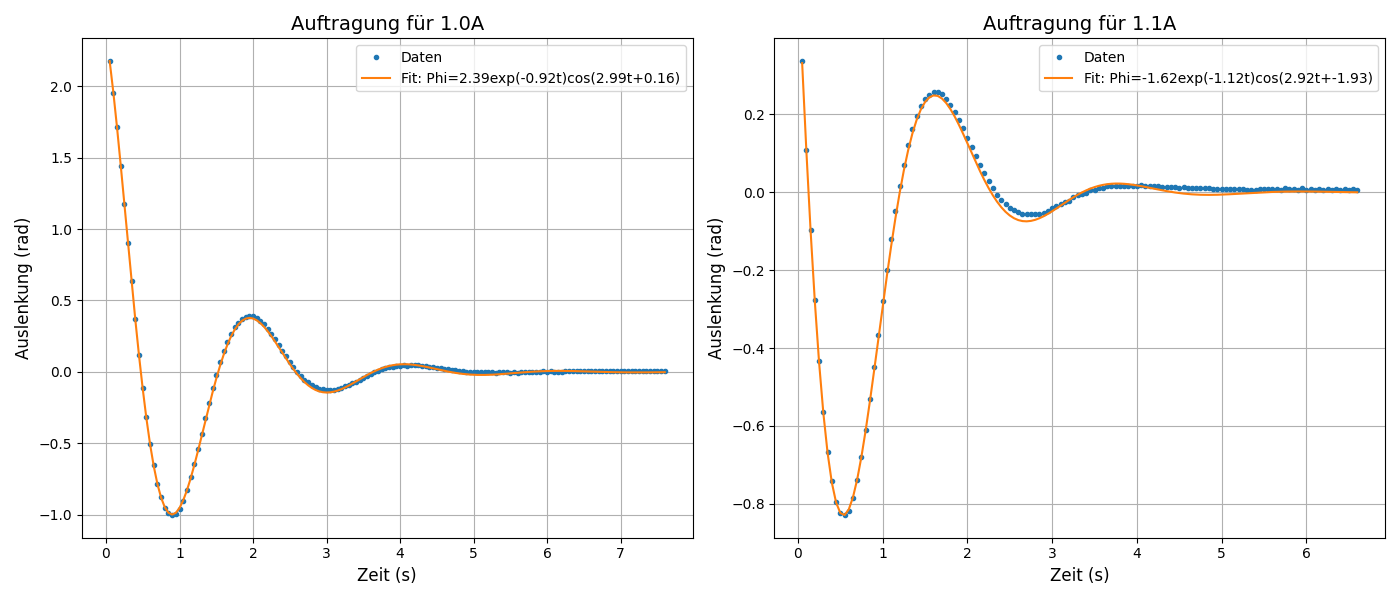
\includegraphics[width=0.85\textwidth]{Figure_5.png}
    \caption{Datenanpassung für Dämpfungsströme (5).}
    \label{fig:5}
\end{figure}
\begin{figure}[H]
    \centering
    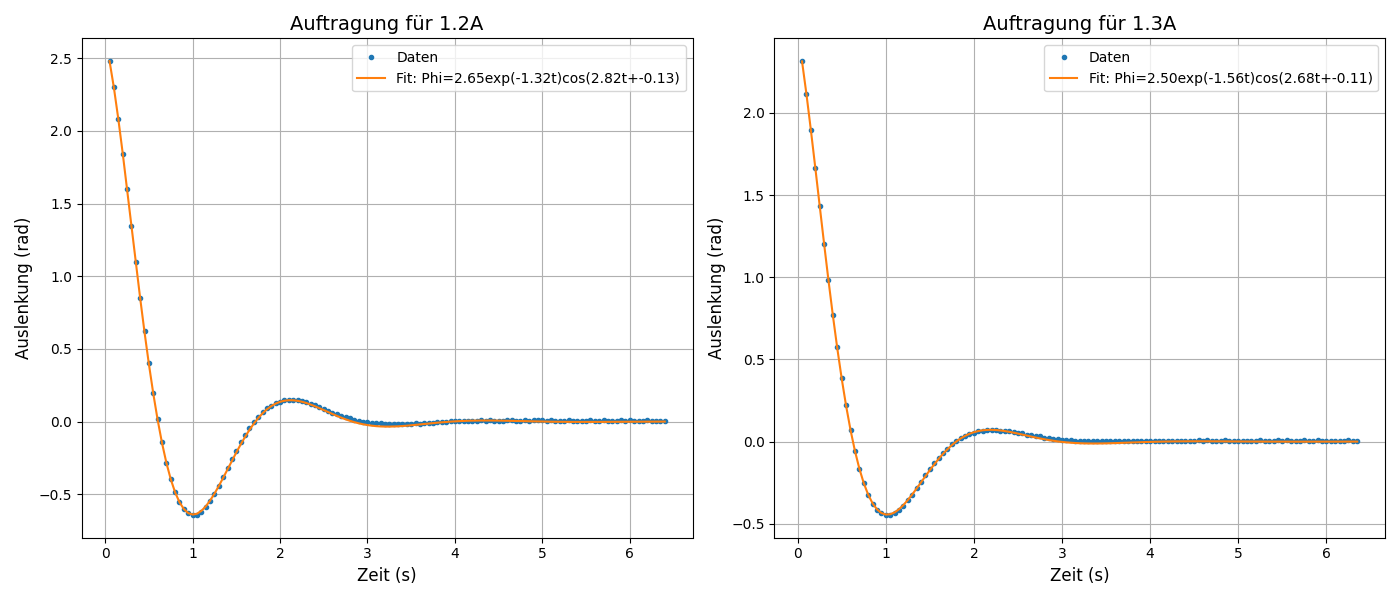
\includegraphics[width=0.85\textwidth]{Figure_6.png}
    \caption{Datenanpassung für Dämpfungsströme (6).}
    \label{fig:6}
\end{figure}
\begin{figure}[H]
    \centering
    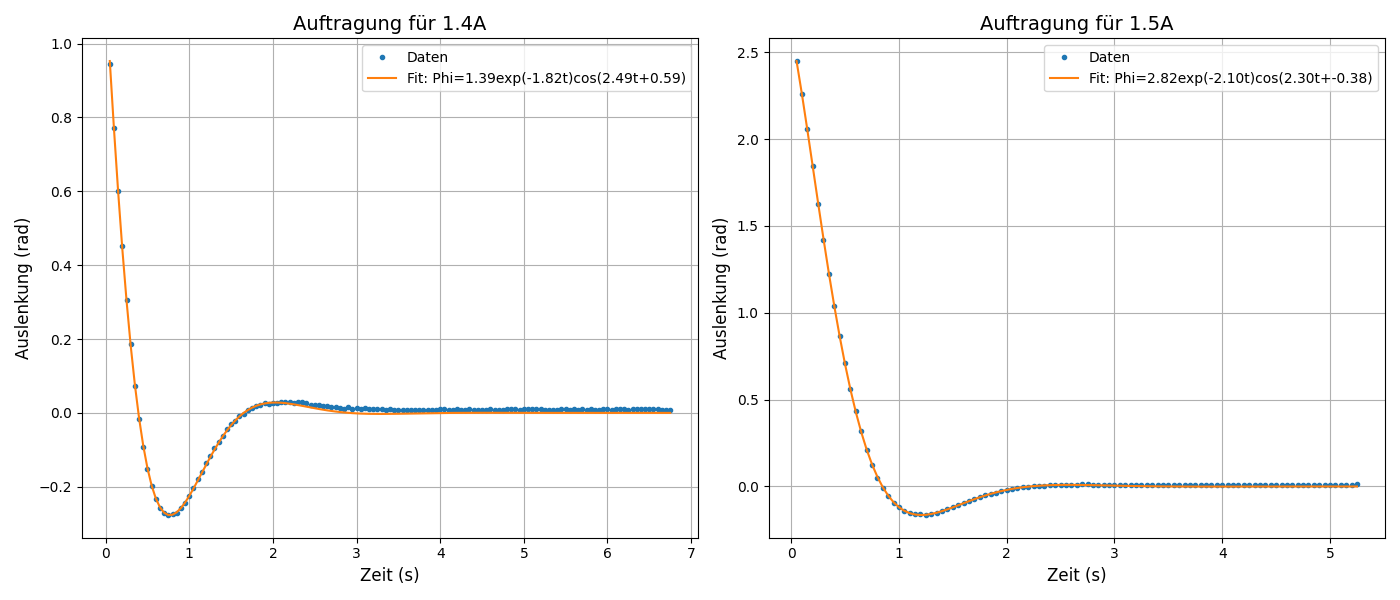
\includegraphics[width=0.85\textwidth]{Figure_7.png}
    \caption{Datenanpassung für Dämpfungsströme (7).}
    \label{fig:7}
\end{figure}

%----------------------------------------------------------------------------------------------------
\clearpage

\addcontentsline{toc}{section}{Literaturverzeichnis}

\begin{thebibliography}{9}

    \bibitem{Versuchsanleitung}
    Technische Universität München, ``Versuchsanleitung POR'', abgerufen am \today,
    [Online]. Verfügbar unter: \url{https://academics.nat.tum.de/fileadmin/w00bzl/nat/studium/org/labs/ph-ap/ap1/POR.pdf}

    \bibitem{Messwerte virtuellen Versuchs}
    Messwerte vom virtuellen Versuch: POR, Dämpfungsstrom 0.35 A. Technische Universität München, abgerufen am \today,
    [Online]. Verfügbar unter: \url{https://view.officeapps.live.com/op/view.aspx?src=https%3A%2F%2Fquintern.xyz%2Fresources%2Fpraktikum%2FPOR_Donat_Quintern.ods&wdOrigin=BROWSELINK}

\end{thebibliography}

\end{document}